\section{Opdracht}
Maak een ontwerp waarmee capaciteit te meten is.

\section{Specificaties}
Het ontwerp moet
\begin{enumerate}
    \item vanaf 10pF kunnen meten
    \item tot 100pF kunnen meten
    \item \dots\% precies zijn
    \item \dots\% nauwkeurig zijn
\end{enumerate}

\begin{figure}
    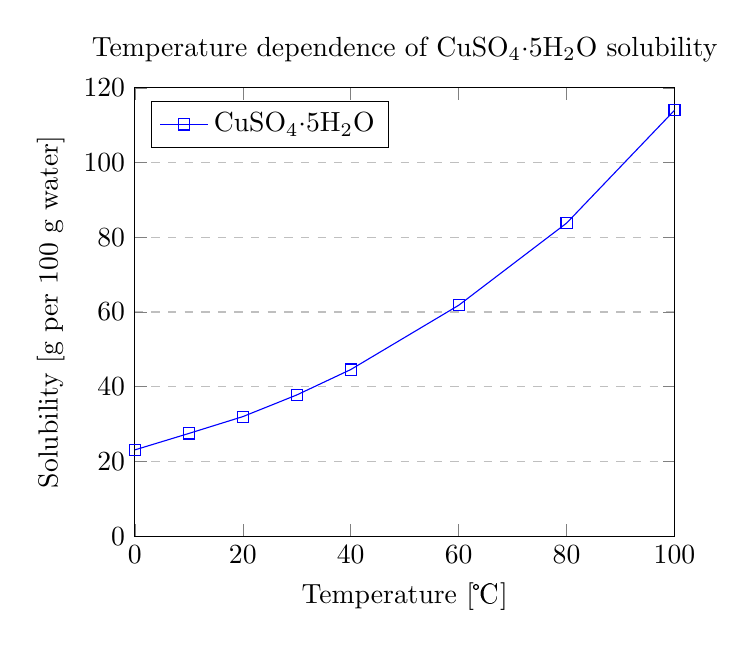
\begin{tikzpicture}
        \begin{axis}[
            title={Temperature dependence of CuSO\(_4\cdot\)5H\(_2\)O solubility},
            xlabel={Temperature [\textcelsius]},
            ylabel={Solubility [g per 100 g water]},
            xmin=0, xmax=100,
            ymin=0, ymax=120,
            xtick={0,20,40,60,80,100},
            ytick={0,20,40,60,80,100,120},
            legend pos=north west,
            ymajorgrids=true,
            grid style=dashed,
        ]
        
        \addplot[
            color=blue,
            mark=square,
            ]
            coordinates {
            (0,23.1)(10,27.5)(20,32)(30,37.8)(40,44.6)(60,61.8)(80,83.8)(100,114)
            };
            \legend{CuSO\(_4\cdot\)5H\(_2\)O}
            
        \end{axis}
    \end{tikzpicture}
\end{figure}